\chapter{OSDOCR Pipeline - Implementação}
\label{cap_osdocr_pipeline_implementacao}

Neste capítulo, será explorada a implementação da componente de pipeline.

De forma a criar um caso de uso para as ferramentas criadas e outras exploradas e disponibilizadas, foi criado um comando de aplicação de uma pipeline de aplicação de OCR, que permite, a partir de uma imagem: aplicar tratamentos para melhorar a sua qualidade; aplicar OCR; tratar os resultados; e gerar um output simples, ou específico para jornais.

Através dos argumentos passados à ferramenta, a pipeline consegue comportar-se de forma diferente, por exemplo: aceitar como output inicial uma instância de Hocr ou de OCR Tree em formato JSON; ignorar pré-processamento ou passos específicos deste; etc.

As funcionalidades disponíveis na pipeline são uma culminação do trabalho descrito anteriormente sobre o OSDOCR Toolkit, assim como ferramentas exploradas para resolver questões que este não aborda como, por exemplo, realização de upscaling de uma imagem.

\section{Sumário}

O comando de invocação da pipeline é 'osdocr'. Este apresenta as seguintes opções de utilização:

\begin{itemize}\setlength\itemsep{-0.8em}
	\item \textbf{target} 
		\begin{itemize}\setlength\itemsep{-0.5em}
			\item \textbf{alternativo} : t
			\item \textbf{descrição} : ficheiro de imagem a ser processado pela pipeline.
		\end{itemize}
		
	\item \textbf{file}
		\begin{itemize}\setlength\itemsep{-0.5em}
			\item \textbf{alternativo} : f
			\item \textbf{descrição} : ficheiro de texto que lista um target por linha.
		\end{itemize}
		
	\item \textbf{target\_ocr\_results} 
		\begin{itemize}\setlength\itemsep{-0.5em}
			\item \textbf{alternativo} : tocr
			\item \textbf{descrição} : ficheiro de resultados OCR. Pode ser de tipo hocr ou json. Se fornecido, não será realizado pré processamento de imagem ou OCR.
		\end{itemize}
		
	\item \textbf{output\_folder}
		\begin{itemize}\setlength\itemsep{-0.5em}
			\item \textbf{alternativo} : of
			\item \textbf{descrição} : caminho para guardar os resultados
		\end{itemize}
		
	
	\item \textbf{segmented\_ocr}
		\begin{itemize}\setlength\itemsep{-0.5em}
			\item \textbf{alternativo} : sgocr
			\item \textbf{descrição} : flag para aplicação de OCR no target será realizada em cada um dos segmentos, invés de na imagem inteira. Cada uma das partes é posteriormente unida para criar uma única OCR Tree de resultados.
			\item \textbf{valor default} : False
		\end{itemize}
		
	\item \textbf{target\_segments}
		\begin{itemize}\setlength\itemsep{-0.5em}
			\item \textbf{alternativo} : ts
			\item \textbf{descrição} : segmentos a calcular no target. Segmento body é sempre obtido. O body é ainda repartido nas suas colunas.
			\item \textbf{opções} : 'header', 'body', 'footer'
			\item \textbf{valor default} : 'header','body'
		\end{itemize}
		
	\item \textbf{force\_ocr}
		\begin{itemize}\setlength\itemsep{-0.5em}
			\item \textbf{alternativo} : focr
			\item \textbf{descrição} : flag que ignora possíveis ficheiros em cache de resultados OCR, consequentes de iterações anteriores do target. Força aplicação de na imagem.
			\item \textbf{valor default} : False
		\end{itemize}
		
	\item \textbf{tesseract\_config}
		\begin{itemize}\setlength\itemsep{-0.5em}
			\item \textbf{descrição} : flags para serem passadas ao Tesseract no momento de aplicação de OCR. Estas estão disponíveis na documentação do Tesseract. Cada argumento tem de ter como prefixo '\_\_' para permitir o seu processamento.
			\item \textbf{valor default} : \_\_l por
		\end{itemize}
	
	\item \textbf{text\_confidence}
		\begin{itemize}\setlength\itemsep{-0.5em}
			\item \textbf{alternativo} : tc
			\item \textbf{descrição} : valor de confiança de texto que pipeline irá usar.
			\item \textbf{valor default} : 10
		\end{itemize}
	
	
	\item \textbf{split\_whitespace}
		\begin{itemize}\setlength\itemsep{-0.5em}
			\item \textbf{alternativo} : sw
			\item \textbf{descrição} : valor utilizado como razão entre um espaço branco num bloco de texto e a média pesada dos espaçamentos entre palavras, para este ser considerado válido como ponto de divisão de um bloco.
			\item \textbf{valor default} : 3
		\end{itemize}
	
	\item \textbf{fix\_rotation}
		\begin{itemize}\setlength\itemsep{-0.5em}
			\item \textbf{alternativo} : fr
			\item \textbf{descrição} : opções usadas para a correção de rotação de documento.
			\item \textbf{opções} : 'auto','clockwise','counter-clockwise'
			\item \textbf{valor default} : 'auto'
		\end{itemize}
	
	\item \textbf{upscaling\_image}
		\begin{itemize}\setlength\itemsep{-0.5em}
			\item \textbf{alternativo} : upi
			\item \textbf{descrição} : opções usadas para o upscaling de imagem. Se opção 'autoscale' do modelo 'waifu2x' for escolhido, aplica upscaling da imagem até esta chegar ao dpi alvo (opção target\_dpi).
			\item \textbf{opções} : 'waifu2x' -> 'scale2x', 'scale4x', 'autoscale'
			\item \textbf{valor default} : 'waifu2x'
		\end{itemize}
	
	\item \textbf{target\_dpi}
		\begin{itemize}\setlength\itemsep{-0.5em}
			\item \textbf{alternativo} : tdpi
			\item \textbf{descrição} : valor do dpi alvo
			\item \textbf{valor default} : 300
		\end{itemize}
	
	\item \textbf{target\_dimensions}
		\begin{itemize}\setlength\itemsep{-0.5em}
			\item \textbf{alternativo} : tdim
			\item \textbf{descrição} : valor das dimensões físicas a usar para cálculo do dpi da imagem. Opções estão disponíveis no ficheiro 'dimensions.json' no projeto, podendo ser atualizado.
			\item \textbf{opções} : 'A5', 'A4', 'A3', 'A2', 'A1', 'A0', '2A0'
			\item \textbf{valor default} : A3
		\end{itemize}
	
	\item \textbf{denoise\_image}
		\begin{itemize}\setlength\itemsep{-0.5em}
			\item \textbf{alternativo} : di
			\item \textbf{descrição} : opções usadas para o denoising de imagem.
			\item \textbf{opções} : 'waifu2x' -> '-1' - '3'
			\item \textbf{valor default} : 'waifu2x'
		\end{itemize}
	
	\item \textbf{light\_correction}
		\begin{itemize}\setlength\itemsep{-0.5em}
			\item \textbf{alternativo} : lc
			\item \textbf{descrição} : opções usadas para a correção de iluminação de uma imagem.
			\item \textbf{opções} : 'best\_SSIM', 'best\_PSNR', 'LOL-Blur', 'SICE', 'SID', 'w\_perc'
			\item \textbf{valor default} : 'best\_SSIM'
		\end{itemize}
		
	\item \textbf{light\_correction\_split\_image}
	\begin{itemize}\setlength\itemsep{-0.5em}
		\item \textbf{alternativo} : lcs
		\item \textbf{descrição} : flag para aplicação de correção de iluminação da imagem em patches, invés de na totalidade, de modo a melhorar tempo de processamento. Para certos modelos, resulta em contrastes consideráveis entre os patches.
		\item \textbf{valor default} : True
	\end{itemize}
	
	\item \textbf{binarize\_image}
		\begin{itemize}\setlength\itemsep{-0.5em}
			\item \textbf{alternativo} : bi
			\item \textbf{descrição} : opções usadas para a binarização de imagem para aplicação de OCR.
			\item \textbf{opções} : 'fax', 'otsu'
			\item \textbf{valor default} : 'fax'
		\end{itemize}
	
	\item \textbf{remove\_document\_images}
		\begin{itemize}\setlength\itemsep{-0.5em}
			\item \textbf{alternativo} : bi
			\item \textbf{descrição} : método utilizado para remoção de imagens.
			\item \textbf{opções} : 'leptonica', 'layoutparser'
			\item \textbf{valor default} : 'leptonica'
		\end{itemize}
	
	\item \textbf{target\_old\_document}
		\begin{itemize}\setlength\itemsep{-0.5em}
			\item \textbf{alternativo} : tod
			\item \textbf{descrição} : flag para indicar que target é um documento antigo. Utilizado quando método 'layoutparser' é escolhido, de forma a escolher o modelo mais apropriado
			\item \textbf{valor default} : True
		\end{itemize}
	
	\item \textbf{ignore\_delimiters}
		\begin{itemize}\setlength\itemsep{-0.5em}
			\item \textbf{alternativo} : igd
			\item \textbf{descrição} : flag para ignorar delimitadores. Se ativada, estes não serão tidos em conta como indicadores do layout do documento no cálculo da ordem de leitura.
			\item \textbf{valor default} : False
		\end{itemize}
	
	\item \textbf{skip\_method}
		\begin{itemize}\setlength\itemsep{-0.5em}
			\item \textbf{descrição} : métodos/passos da pipeline a ignorar.
			\item \textbf{opções} : 'leptonica', 'layoutparser'
			\item \textbf{valor default} : 'all', 'auto\_rotate', 'noise\_removal', 'blur\_removal', 'light\_correction', 'image\_preprocess', 'remove\_document\_margins', 'remove\_document\_images', 'image\_upscaling', 'identify\_document\_delimiters', 'binarize\_image', 'clean\_ocr', 'split\_whitespace', 'unite\_blocks', 'calculate\_reading\_order', 'extract\_articles', 'posprocessing'
		\end{itemize}
	
	\item \textbf{calibrate}
		\begin{itemize}\setlength\itemsep{-0.5em}
			\item \textbf{descrição} : aplicar modo de calibração de pipeline. Usado para encontrar melhor configuração de pipeline para um dado target. Pode ser dado um diretório onde estarão disponíveis os ficheiros necessários para calibração, e onde ficarão os resultados de calibração; e um diretório com configurações de pipeline a testar. Por defeito, o diretório procurado dá-se por 'calibration' no local onde o comando foi corrido, e são usadas configurações de pipeline disponíveis no projeto. 
		\end{itemize}
	
	\item \textbf{calibrate\_no\_reuse}
		\begin{itemize}\setlength\itemsep{-0.5em}
			\item \textbf{descrição} : flag para não utilizar cache existente.
			\item \textbf{valor default} : False
		\end{itemize}
	
	\item \textbf{pipeline\_config}
		\begin{itemize}\setlength\itemsep{-0.5em}
			\item \textbf{descrição} : ficheiro do tipo JSON com configuração de pipeline a usar. Pode ser usado como alternativa a aplicar argumentos no terminal de comandos.
		\end{itemize}
		
	\item \textbf{gui}
		\begin{itemize}\setlength\itemsep{-0.5em}
			\item \textbf{descrição} : aplicar modo de interface gráfica. Interface gráfica simples que pode ser utilizada para experimentar algumas das funcionalidades disponíveis. Maioritariamente usada para debugging.
		\end{itemize}
\end{itemize}


\section{Pré-processamento de imagem}

Como primeiro procedimento da pipeline, no caso de uso de inputs de imagem, tem-se o tratamento desta, para procurar obter, a partir da aplicação OCR, uma melhor transcrição do conteúdo textual, assim como melhor identificação de outros elementos, como figuras.

Para isso, procurou-se abordar os seguintes problemas: imagens rodadas; remoção de margens/sombras na margem de documentos; imagens de baixa resolução; remoção de figuras de documentos; imagens com ruído; imagens com distribuição de iluminação inconsistente;.

As solução destes problemas envolveram o uso de métodos desenvolvidos no toolkit, assim como soluções já existentes.

A ordem de aplicação destas soluções mostrou ser relevante pois estas podem interferir umas com as outras, por exemplo: aplicação de denoising antes de remover as figuras do documento pode afetar a identificação destas. Assim sendo, a ordem ótima de execução segue a listagem que se segue.

\begin{figure}[H]
	\centering
	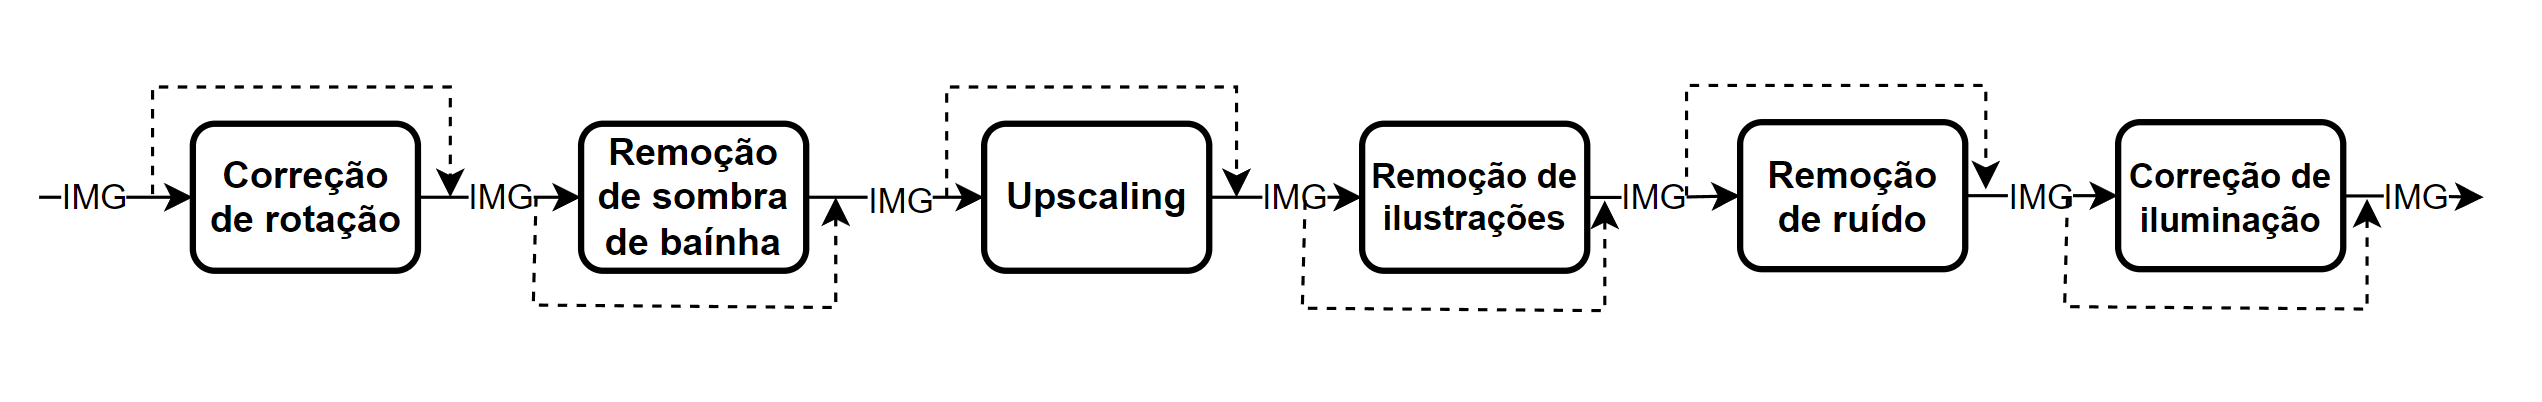
\includegraphics[width=1\textwidth]{images/diagramas/arquitetura_pipeline_preprocess.png}
	\caption{Pipeline - secção pré-processamento}
	\label{fig:arquitetura_pipeline_preprocess}
\end{figure}

\highlight{Correção de rotação}

A correção de possíveis rotações de imagens de documentos é resolvida utilizando os métodos de correção de rotação descritos na secção de métodos de processamento de imagem.

\highlight{Remoção de sombras das margens do documento}

De igual modo, a remoção de possíveis sombras na margem de um documento aproveita os métodos desenvolvidos e descritos para este efeito na mesma secção. 

A aplicação desta funcionalidade deve vir após a correção de possíveis rotações pois, como esta solução envolve a análise da distribuição dos valores de pixeis, se estas sombras se apresentarem inclinadas a possibilidade que elas não sejam resolvidas aumenta.


\highlight{Upscaling de imagem}

Para a resolução de problemas resultantes de imagens com baixos valores de dpi, modelos de Deep Learning obtém resultados mais interessantes em relação a algoritmos passados, como interpolação. Dentro destes modelos, o \href{https://github.com/nagadomi/waifu2x}{waifu2x} é bastante respeitado no que toca a aumento de resolução de imagem e limpeza de imperfeições. 

Embora não especificamente focado para o processamento de imagens de documentos, o seu fácil uso e instalação, assim como a verificação de bons resultados mesmo nesta área relativamente externa ao treino, levaram a que este modelo seja uma boa adição às ferramentas de pré-processamento de imagem disponíveis na pipeline.

Esta funcionalidade, quando escolhida para realizar upscaling automático, é dependente das configurações utilizadas para cálculo de dpi de imagem (dimensões reais proporcionadas).

A aplicação de OCR é recomendada para dpi no valor de 300 ou superior, sendo que para imagens antigas, esta funcionalidade é essencial.

%% TODO : ilustracao de upscaling. zoom numa parte de imagem com e sem upscaling


\highlight{Remoção de ilustrações de documento}

De forma a diminuir a presença de elementos não identificados nos resultados OCR, assim como permitir identifica-los corretamente, esta funcionalidade procura remover as ilustrações de um documento, recortando-as para uma pasta temporário, permitindo a sua reposição na imagem final.

Entre as soluções exploradas para esta questão, a que se enquadrava mais na questão de identificação de ilustrações de documentos, e até com atenção a jornais, foi o modelo \href{https://layout-parser.readthedocs.io/en/latest/index.html}{Layout Parser}, mais especificamente, aproveitando o modelo Detectron desenvolvido pela Meta.
Este, no entanto, apresenta uma instalação complexa devido a dependências de bibliotecas da própria Meta que demonstram incompatibilidades e que necessitam ser modificadas manualmente.

Deste modo, aproveitou-se uma alternativa com resultados também satisfatórios e de menor custo computacional, com métodos de segmentação de documento propostos pela Leptonica. Estes foram descritos também na secção anterior.

Comparando os dois, a opção de usar Leptonica é satisfatória na generalidade dos casos, até identificando com maior precisão as ilustrações (delimitando menos fundo do documento) em vários casos de estudo. Os métodos de Leptonica tendem no entanto a errar para ilustrações que não apresentem uma borda notável e tenham um fundo similar ao fundo do documento. Nestes casos, o Layout Parser é mais propício a acertar.

%% TODO : ilustracao de ilustrações removidas de um documento

É também importante realçar que a pipeline, no processo de recortar as ilustrações, preenche o espaço vazio com uma média das cores de fundo da imagem. Este passo é importante pois caso contrário a binarização posterior da imagem, dependendo da distribuição das cores desta, pode resultar numa imagem inutilizável.

%% TODO : ilustracao de binarizacao nos dois casos de remocao de ilustracoes

\highlight{Denoising de imagem}

Para a realização de denoising, foi também aplicado o modelo de \textbf{waifu2x}, visto este proporcionar opções para este efeito. Este denoising é realizado em imagens a cor, sendo portanto subtil.

O denoising mais relevante é realizado na binarização realizada antes da aplicação de OCR.

%% TODO : ilustracao de denoising.


\highlight{Correção de iluminação}

Para a correção de iluminação de documentos, também se conclui que modelos de Deep Learning são a melhor opção. A família de modelos que mostraram resultados mais interessantes foi \href{https://github.com/Fediory/HVI-CIDNet}{HVI-CIDNet}, Os pesos para estes estão disponibilizados nesse mesmo repositório.

Para imagens de maior resolução, o tempo de processamento destes modelos é considerável, sendo que como solução a pipeline apresenta uma opção para dividir a imagem em patches e correr o modelo em cada um destes, unindo-os no final. Para alguns modelos, esta divisão pode resultar em contrastes notáveis na imagem

%% TODO : ilustracao de correcao de iluminacao utilizando diferentes modelos

%% TODO : ilustracao de correcao de iluminacao com e sem patches


\section{OCR}


Seguindo na pipeline, temos a a aplicação de OCR para extração do conteúdo textual de uma imagem. No caso de input do tipo OCR Tree - ou seu convertível -, este passo é ignorado, caso contrário é obrigatório.

% OCR de imagem

Ao longo da implementação e estudo dos resultados desta, foi utilizado \textbf{Tesseract} para a realização de OCR, devido a ser uma ferramenta open-source no topo do estado da arte.

O processo de OCR da pipeline pode ser dividido em blocos menores, sendo estes:

%% TODO ilustracao : diagrama de blocos da seccao de OCR


\highlight{Binarização}

%% binarizacao

A binarização de imagem é um processo que permite a realização de redução de ruído através da aplicação de tresholds, assim como a acentuação do texto de documentos. Este passo é também recomendado na documentação do Tesseract..

Este passo pode ser ignorado na pipeline, até pois o Tesseract internamente irá aplicar uma binarização própria.

A pipeline apresenta a opção de realizar binarização utilizando \textbf{Otsu} ou estilo \textbf{Fax}.

\begin{figure}[H]
	\centering
	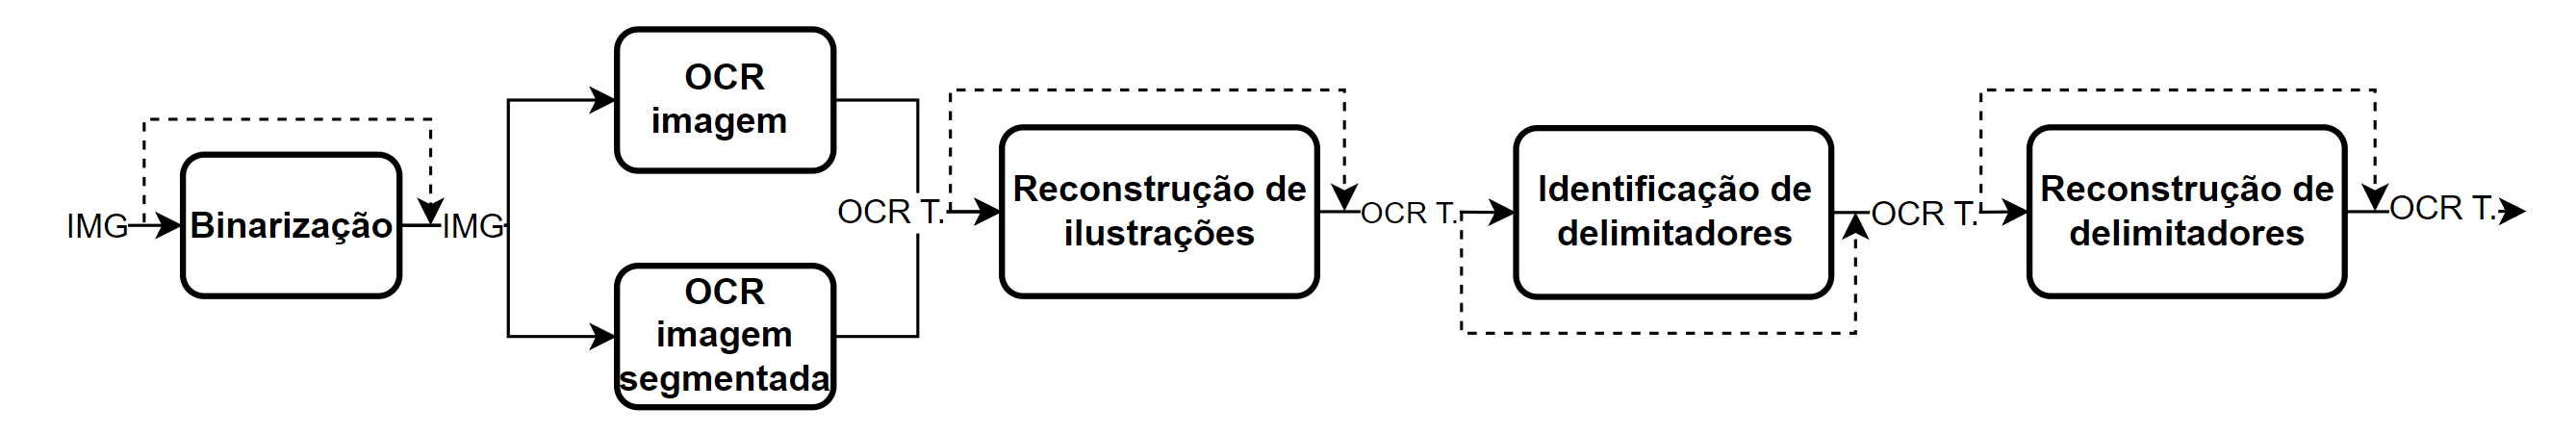
\includegraphics[width=1\textwidth]{images/diagramas/arquitetura_pipeline_ocr.png}
	\caption{Pipeline - secção OCR}
	\label{fig:arquitetura_pipeline_ocr}
\end{figure}



\highlight{OCR em imagem}

%%% imagem simples

A aplicação de OCR é realizada utilizando \textbf{Tesseract} podendo, através dos argumentos da pipeline, modificar a configuração deste, por exemplo: linguagem do texto a detetar; dpi da imagem; modo de segmentação.

Os resultados de OCR serão transformados numa OCR Tree.

\highlight{OCR em imagem segmentada}

%%% imagem segmentada

Em muitos casos, os documentos antigos apresentam variações do seu estado ao longo do documento. Por este motivo, a pipeline permite a habilidade de realizar um reconhecimento de texto aos diferentes segmentos da imagem, invés de numa única passagem. 

Para isto, podem ser passados os segmentos esperados na consola: 'header' , 'body' e 'footer'. Utilizando métodos de processamento de imagem do Toolkit, o documento será dividido nestes segmentos, particularmente o body será possivelmente ainda dividido em colunas, que serão separadamente binarizados (se intendido) e analisados com OCR.

Em seguida as diferentes OCR Tree resultantes serão unidas numa única.


\highlight{Reconstrução de delimitadores e imagens nos resultados}

%% incluir imagens e delimitadores identificados

Com a OCR Tree obtida, o último passo desta secção passa pela reconstrução de elementos não textuais do documento na OCR Tree. 

Estes são: ilustrações reconhecidas durante o pré-processamento; delimitadores identificados utilizando o Toolkit (se intendido).

Os elementos serão adicionados na OCR Tree, removendo blocos vazios que se situem dentro ou a intersetar com estes novos elementos.



\section{Pós-processamento de OCR}

% tratamento de resultados
%% clean OCR
%% categorizacao OCR
%% Uniao OCR
%% Find titles TODO : nao falado anteriormente

\section{Geração de output}

% criacao de output
%% output para jornal
%%% calculo da ordem de leitura
%%% output para text
%%% output para markdown
%% output simples
%%% output text

\section{Validação de resultados}

% validacao de resultados/pipeline





